\documentclass{standalone}%
\usepackage[T1]{fontenc}%
\usepackage[utf8]{inputenc}%
\usepackage{lmodern}%
\usepackage{textcomp}%
\usepackage{lastpage}%
\usepackage{tikz}%
%
%
%
\begin{document}%
\normalsize%
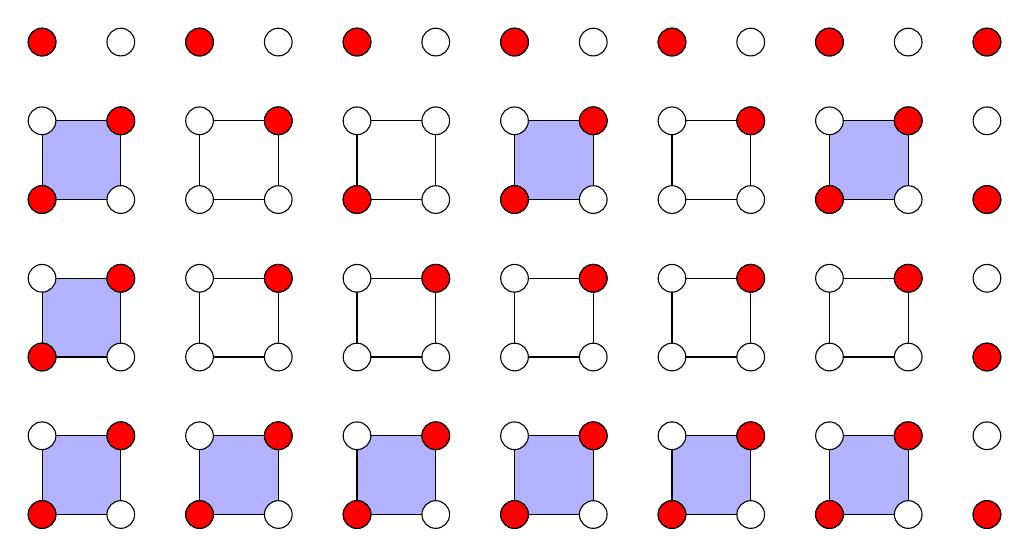
\begin{tikzpicture}[scale=1.0]%
\foreach \x in {0,...,5}
	\foreach \y in {0,...,-2}
		\draw[] (2*\x,2*\y-1) -- (2*\x+1,2*\y-1) -- (2*\x+1,2*\y-2) -- (2*\x,2*\y-2) -- cycle;
\foreach \x in {0,...,5}
	\foreach \y in {-2}
		\draw[fill=blue!30] (2*\x,2*\y-1) rectangle (2*\x+1,2*\y-2);
\draw[fill=blue!30] (0,-4) rectangle (1,-3);
\draw[fill=blue!30] (0,-2) rectangle (1,-1);
\draw[fill=blue!30] (6,-2) rectangle (7,-1);
\draw[fill=blue!30] (10,-2) rectangle (11,-1);

\path[draw,radius=5pt, fill=white] (0.0,0.0) circle;%
\path[draw,radius=5pt, fill=white] (1.0,0.0) circle;%
\path[draw,radius=5pt, fill=white] (2.0,0.0) circle;%
\path[draw,radius=5pt, fill=white] (3.0,0.0) circle;%
\path[draw,radius=5pt, fill=white] (4.0,0.0) circle;%
\path[draw,radius=5pt, fill=white] (5.0,0.0) circle;%
\path[draw,radius=5pt, fill=white] (6.0,0.0) circle;%
\path[draw,radius=5pt, fill=white] (7.0,0.0) circle;%
\path[draw,radius=5pt, fill=white] (8.0,0.0) circle;%
\path[draw,radius=5pt, fill=white] (9.0,0.0) circle;%
\path[draw,radius=5pt, fill=white] (10.0,0.0) circle;%
\path[draw,radius=5pt, fill=white] (11.0,0.0) circle;%
\path[draw,radius=5pt, fill=white] (12.0,0.0) circle;%
\path[draw,radius=5pt, fill=white] (0.0,-1.0) circle;%
\path[draw,radius=5pt, fill=white] (1.0,-1.0) circle;%
\path[draw,radius=5pt, fill=white] (2.0,-1.0) circle;%
\path[draw,radius=5pt, fill=white] (3.0,-1.0) circle;%
\path[draw,radius=5pt, fill=white] (4.0,-1.0) circle;%
\path[draw,radius=5pt, fill=white] (5.0,-1.0) circle;%
\path[draw,radius=5pt, fill=white] (6.0,-1.0) circle;%
\path[draw,radius=5pt, fill=white] (7.0,-1.0) circle;%
\path[draw,radius=5pt, fill=white] (8.0,-1.0) circle;%
\path[draw,radius=5pt, fill=white] (9.0,-1.0) circle;%
\path[draw,radius=5pt, fill=white] (10.0,-1.0) circle;%
\path[draw,radius=5pt, fill=white] (11.0,-1.0) circle;%
\path[draw,radius=5pt, fill=white] (12.0,-1.0) circle;%
\path[draw,radius=5pt, fill=white] (0.0,-2.0) circle;%
\path[draw,radius=5pt, fill=white] (1.0,-2.0) circle;%
\path[draw,radius=5pt, fill=white] (2.0,-2.0) circle;%
\path[draw,radius=5pt, fill=white] (3.0,-2.0) circle;%
\path[draw,radius=5pt, fill=white] (4.0,-2.0) circle;%
\path[draw,radius=5pt, fill=white] (5.0,-2.0) circle;%
\path[draw,radius=5pt, fill=white] (6.0,-2.0) circle;%
\path[draw,radius=5pt, fill=white] (7.0,-2.0) circle;%
\path[draw,radius=5pt, fill=white] (8.0,-2.0) circle;%
\path[draw,radius=5pt, fill=white] (9.0,-2.0) circle;%
\path[draw,radius=5pt, fill=white] (10.0,-2.0) circle;%
\path[draw,radius=5pt, fill=white] (11.0,-2.0) circle;%
\path[draw,radius=5pt, fill=white] (12.0,-2.0) circle;%
\path[draw,radius=5pt, fill=white] (0.0,-3.0) circle;%
\path[draw,radius=5pt, fill=white] (1.0,-3.0) circle;%
\path[draw,radius=5pt, fill=white] (2.0,-3.0) circle;%
\path[draw,radius=5pt, fill=white] (3.0,-3.0) circle;%
\path[draw,radius=5pt, fill=white] (4.0,-3.0) circle;%
\path[draw,radius=5pt, fill=white] (5.0,-3.0) circle;%
\path[draw,radius=5pt, fill=white] (6.0,-3.0) circle;%
\path[draw,radius=5pt, fill=white] (7.0,-3.0) circle;%
\path[draw,radius=5pt, fill=white] (8.0,-3.0) circle;%
\path[draw,radius=5pt, fill=white] (9.0,-3.0) circle;%
\path[draw,radius=5pt, fill=white] (10.0,-3.0) circle;%
\path[draw,radius=5pt, fill=white] (11.0,-3.0) circle;%
\path[draw,radius=5pt, fill=white] (12.0,-3.0) circle;%
\path[draw,radius=5pt, fill=white] (0.0,-4.0) circle;%
\path[draw,radius=5pt, fill=white] (1.0,-4.0) circle;%
\path[draw,radius=5pt, fill=white] (2.0,-4.0) circle;%
\path[draw,radius=5pt, fill=white] (3.0,-4.0) circle;%
\path[draw,radius=5pt, fill=white] (4.0,-4.0) circle;%
\path[draw,radius=5pt, fill=white] (5.0,-4.0) circle;%
\path[draw,radius=5pt, fill=white] (6.0,-4.0) circle;%
\path[draw,radius=5pt, fill=white] (7.0,-4.0) circle;%
\path[draw,radius=5pt, fill=white] (8.0,-4.0) circle;%
\path[draw,radius=5pt, fill=white] (9.0,-4.0) circle;%
\path[draw,radius=5pt, fill=white] (10.0,-4.0) circle;%
\path[draw,radius=5pt, fill=white] (11.0,-4.0) circle;%
\path[draw,radius=5pt, fill=white] (12.0,-4.0) circle;%
\path[draw,radius=5pt, fill=white] (0.0,-5.0) circle;%
\path[draw,radius=5pt, fill=white] (1.0,-5.0) circle;%
\path[draw,radius=5pt, fill=white] (2.0,-5.0) circle;%
\path[draw,radius=5pt, fill=white] (3.0,-5.0) circle;%
\path[draw,radius=5pt, fill=white] (4.0,-5.0) circle;%
\path[draw,radius=5pt, fill=white] (5.0,-5.0) circle;%
\path[draw,radius=5pt, fill=white] (6.0,-5.0) circle;%
\path[draw,radius=5pt, fill=white] (7.0,-5.0) circle;%
\path[draw,radius=5pt, fill=white] (8.0,-5.0) circle;%
\path[draw,radius=5pt, fill=white] (9.0,-5.0) circle;%
\path[draw,radius=5pt, fill=white] (10.0,-5.0) circle;%
\path[draw,radius=5pt, fill=white] (11.0,-5.0) circle;%
\path[draw,radius=5pt, fill=white] (12.0,-5.0) circle;%
\path[draw,radius=5pt, fill=white] (0.0,-6.0) circle;%
\path[draw,radius=5pt, fill=white] (1.0,-6.0) circle;%
\path[draw,radius=5pt, fill=white] (2.0,-6.0) circle;%
\path[draw,radius=5pt, fill=white] (3.0,-6.0) circle;%
\path[draw,radius=5pt, fill=white] (4.0,-6.0) circle;%
\path[draw,radius=5pt, fill=white] (5.0,-6.0) circle;%
\path[draw,radius=5pt, fill=white] (6.0,-6.0) circle;%
\path[draw,radius=5pt, fill=white] (7.0,-6.0) circle;%
\path[draw,radius=5pt, fill=white] (8.0,-6.0) circle;%
\path[draw,radius=5pt, fill=white] (9.0,-6.0) circle;%
\path[draw,radius=5pt, fill=white] (10.0,-6.0) circle;%
\path[draw,radius=5pt, fill=white] (11.0,-6.0) circle;%
\path[draw,radius=5pt, fill=white] (12.0,-6.0) circle;%
\path[draw,radius=5pt,fill=red] (0.0,0.0) circle;%
\path[draw,radius=5pt,fill=red] (2.0,0.0) circle;%
\path[draw,radius=5pt,fill=red] (4.0,0.0) circle;%
\path[draw,radius=5pt,fill=red] (6.0,0.0) circle;%
\path[draw,radius=5pt,fill=red] (8.0,0.0) circle;%
\path[draw,radius=5pt,fill=red] (10.0,0.0) circle;%
\path[draw,radius=5pt,fill=red] (12.0,0.0) circle;%
\path[draw,radius=5pt,fill=red] (1.0,-1.0) circle;%
\path[draw,radius=5pt,fill=red] (3.0,-1.0) circle;%
\path[draw,radius=5pt,fill=red] (7.0,-1.0) circle;%
\path[draw,radius=5pt,fill=red] (9.0,-1.0) circle;%
\path[draw,radius=5pt,fill=red] (11.0,-1.0) circle;%
\path[draw,radius=5pt,fill=red] (0.0,-2.0) circle;%
\path[draw,radius=5pt,fill=red] (4.0,-2.0) circle;%
\path[draw,radius=5pt,fill=red] (6.0,-2.0) circle;%
\path[draw,radius=5pt,fill=red] (10.0,-2.0) circle;%
\path[draw,radius=5pt,fill=red] (12.0,-2.0) circle;%
\path[draw,radius=5pt,fill=red] (1.0,-3.0) circle;%
\path[draw,radius=5pt,fill=red] (3.0,-3.0) circle;%
\path[draw,radius=5pt,fill=red] (5.0,-3.0) circle;%
\path[draw,radius=5pt,fill=red] (7.0,-3.0) circle;%
\path[draw,radius=5pt,fill=red] (9.0,-3.0) circle;%
\path[draw,radius=5pt,fill=red] (11.0,-3.0) circle;%
\path[draw,radius=5pt,fill=red] (0.0,-4.0) circle;%
\path[draw,radius=5pt,fill=red] (12.0,-4.0) circle;%
\path[draw,radius=5pt,fill=red] (1.0,-5.0) circle;%
\path[draw,radius=5pt,fill=red] (3.0,-5.0) circle;%
\path[draw,radius=5pt,fill=red] (5.0,-5.0) circle;%
\path[draw,radius=5pt,fill=red] (7.0,-5.0) circle;%
\path[draw,radius=5pt,fill=red] (9.0,-5.0) circle;%
\path[draw,radius=5pt,fill=red] (11.0,-5.0) circle;%
\path[draw,radius=5pt,fill=red] (0.0,-6.0) circle;%
\path[draw,radius=5pt,fill=red] (2.0,-6.0) circle;%
\path[draw,radius=5pt,fill=red] (4.0,-6.0) circle;%
\path[draw,radius=5pt,fill=red] (6.0,-6.0) circle;%
\path[draw,radius=5pt,fill=red] (8.0,-6.0) circle;%
\path[draw,radius=5pt,fill=red] (10.0,-6.0) circle;%
\path[draw,radius=5pt,fill=red] (12.0,-6.0) circle;%
\end{tikzpicture}%
\end{document}